\documentclass{beamer}
\usepackage{beamerthemesplit}
\usetheme{Boadilla}
\usecolortheme{}
\RequirePackage{amssymb}
\RequirePackage{amsfonts}
\RequirePackage{amsmath}
\usepackage{graphicx}			% package to include pdf graphics
\usepackage{fancyhdr}			% gives headers see below
\usepackage{geometry}			% package to give easy control of paper and margin size
\usepackage{latexsym}
\usepackage{color}
\usepackage{amsbsy}
\usepackage{tikz}
\usetikzlibrary{positioning}
\setbeamertemplate{items}[ball]
\usepackage{mathtools}
\usepackage{tikz}
\usetikzlibrary{%
  matrix,%
  calc,%
  arrows%
}

\beamertemplatenavigationsymbolsempty

%------ New Commands ------%

\newcommand{\R}[1]{\mathbb{R}^{#1}}
\newcommand{\Z}[1]{\mathbb{Z}^{#1}}
\newcommand{\im}{\mbox{im}}
\newcommand{\omg}[1]{\boldsymbol{\Omega}^{#1}}
\newcommand{\pd}[2]{\frac{\partial#1}{\partial#2}}

%------------------------------------%

\title{Topics In Equivariant Cohomology}
\subtitle{Or: How I Learned To Stop Worrying And Love Group Actions}
\author[L. Keating Hughes]{Luke Keating Hughes}
\institute[UofA]{
Supervised by Prof. Michael Murray \& Dr. Danny Stevenson\\
University of Adelaide\\
Major Review\\}
\date{27/02/15}


\begin{document}

%--- the titlepage frame -------------------------%
\begin{frame}[plain]
  \titlepage
\end{frame}

%--- the presentation begins here ----------------%





\begin{frame}{Outline}
\begin{itemize}
\item Introduction
\item Basic de Rham Theory
\item Equivariant cohomology
\item Simplicial methods
\item An important example


\end{itemize}
\end{frame}



\begin{frame}{Algebraic Topology}
Algebraic topology is a branch of mathematics that studies spaces by assigning algebraic \emph{invariants} to them.

\begin{exampleblock}{Example: Euler characteristic of a surface}
Take a surface, $S$, embedded in $\R{3}$ and triangulate it. Let $v$ be the number of vertices, $e$ be the number of edges and $f$ be the number of faces of the triangulation. Then $\chi(S)= v - e + f$ is defined to be the Euler characteristic of $S$.
\begin{center}
\includegraphics[scale=0.05]{triangulation2}
\end{center}
\end{exampleblock}
\emph{Cohomology} is a \emph{more refined} algebraic invariant than the Euler characteristic.
\end{frame}



\begin{frame}{What is cohomology?}
For those without any background in algebraic topology, a cohomology theory can be thought of as assigning a sequence of algebraic objects to a topological space.
\[
\mbox{Topological Spaces} \xrightarrow{~~H^{*}~~} \mbox{Algebraic Objects}
\]
Sometimes it is possible to prove results about topological spaces by reducing it to an algebraic problem.
\end{frame}



\begin{frame}{Example: Singular Cohomology}
One example we can consider is \emph{singular cohomology} (with real coefficients).
\begin{align*}
\mbox{Topological Spaces} ~~ &\xrightarrow{~~H^{*}~~} ~~ \mbox{Vector Spaces}~~~~~~~~~~~\\
\\
X ~~~~~~~~ &\xmapsto{~~~~~~~} ~~ H^{0}(X),\ H^{1}(X),\cdots
\end{align*}
Singular cohomology is more refined than the Euler Characteristic.
\[
\chi(X) = dim(H^{0}(X)) - dim(H^{1}(X)) + dim(H^{2}(X)) - \cdots
\]
\end{frame}



\begin{frame}{Basic cohomology theory}
Let $C=\{C_i\}_{i\in\Z{}}$ be a sequence of vector spaces (or more generally, \emph{modules}) and $\delta_{i}:C_i \to C_{i+1}$ be maps such that $\delta_{i+1}\!\circ\delta_{i}=0$. We call this a \emph{cochain complex}.

\begin{center}
\begin{tikzpicture}[scale=0.8, every node/.style={scale=0.8}]
\node (ldots) at (-5,0) {$\cdots$};
\node (C0) at (-3,0) {$C_{i-1}$};
\node (C1) at (-1,0) {$C_{i}$};
\node (C2) at (1,0) {$C_{i+1}$};
\node (C3) at (3,0) {$C_{i+2}$};
\node (C4) at (5,0) {$C_{i+3}$};
\node (rdots) at (7,0) {$\cdots$};

\draw
	(ldots) edge[->] (C0)
	(C0) edge[->] node[auto]{$\delta_{i-1}$} (C1)
	(C1) edge[->] node[auto]{$\delta_{i}$} (C2)
	(C2) edge[->] node[auto]{$\delta_{i+1}$} (C3)
	(C3) edge[->] node[auto]{$\delta_{i+2}$} (C4)
	(C1) edge[->, bend left=45] node[above]{$0$} (C3)
	(C4) edge[->] (rdots)
;
\end{tikzpicture}
\end{center}

\begin{block}{Note}
Saying $\delta_{i+1}\!\circ\delta_{i}=0$ is equivalent to saying that $\im(\delta_{i}) \subset \ker(\delta_{i+1})$. We say the complex is \emph{exact} if $\im(\delta_{i}) = \ker(\delta_{i+1})$ for every $i \in \Z{}$.
\end{block}

Define the \emph{$q^{th}$ cohomology group} of the complex C to be
\begin{align*}
H^{q}(C)=\frac{\ker(\delta_{q}:C_{q} \to C_{q+1})}{\im(\delta_{q-1}:C_{q-1} \to C_{q})}.
\end{align*}
\end{frame}



\begin{frame}{Basic cohomology theory}
Sometimes these cochain complexes can be rather abstract

\begin{center}
\begin{tikzpicture}[scale=0.8, every node/.style={scale=0.8}]
\node (ldots) at (-5,0) {$\cdots$};
\node (C0) at (-3,0) {$\Z{}$};
\node (C1) at (-1,0) {$\Z{}$};
\node (C2) at (1,0) {$\Z{}$};
\node (C3) at (3,0) {$\Z{}$};
\node (C4) at (5,0) {$\Z{}$};
\node (rdots) at (7,0) {$\cdots$};

\draw
	(ldots) edge[->] (C0)
	(C0) edge[->] node[auto]{$\times 2$} (C1)
	(C1) edge[->] node[auto]{$\times 0$} (C2)
	(C2) edge[->] node[auto]{$\times 2$} (C3)
	(C3) edge[->] node[auto]{$\times 0$} (C4)
	(C1) edge[->, bend left=45] node[above]{$0$} (C3)
	(C4) edge[->] (rdots)
;
\end{tikzpicture}
\end{center}

or things we've seen before like \emph{grad}, \emph{curl} and \emph{div}.

\begin{center}
\begin{tikzpicture}[scale=0.8, every node/.style={scale=0.8}]
\node (C0) at (-6,0) {$\bigg\{\parbox{5.8em}{\centering functions from $\R{3}$ to $\R{}$}\bigg\}$};
\node (C1) at (-2,0) {$\bigg\{\parbox{5.8em}{\centering vector fields on $\R{3}$}\bigg\}$};
\node (C2) at (2,0) {$\bigg\{\parbox{5.8em}{\centering vector fields on $\R{3}$}\bigg\}$};
\node (C3) at (6,0) {$\bigg\{\parbox{5.8em}{\centering functions from $\R{3}$ to $\R{}$}\bigg\}$};

\draw
	(C0) edge[->] node[auto]{$\nabla$} (C1)
	(C1) edge[->] node[auto]{$\nabla\times$} (C2)
	(C2) edge[->] node[auto]{$\nabla\boldsymbol{\cdot}$} (C3)
	(C0) edge[->, bend left=35] node[above]{$\nabla\!\times\circ\,\nabla=0$} (C2)
	(C1) edge[->, bend right=35] node[below]{$\nabla\!\boldsymbol{\cdot}\circ\,\nabla\!\times=0$} (C3)
;
\end{tikzpicture}
\end{center}
\end{frame}



\begin{frame}{Example: Multivariable Calculus}
We'll call this complex $V$.
\begin{center}
\begin{tikzpicture}[scale=0.8, every node/.style={scale=0.8}]
\node (C0) at (-6,0) {$\bigg\{\parbox{5.8em}{\centering functions from $\R{3}$ to $\R{}$}\bigg\}$};
\node (C1) at (-2,0) {$\bigg\{\parbox{5.8em}{\centering vector fields on $\R{3}$}\bigg\}$};
\node (C2) at (2,0) {$\bigg\{\parbox{5.8em}{\centering vector fields on $\R{3}$}\bigg\}$};
\node (C3) at (6,0) {$\bigg\{\parbox{5.8em}{\centering functions from $\R{3}$ to $\R{}$}\bigg\}$};

\node (V0) at (-6,-1) {$V_0$};
\node (V1) at (-2,-1) {$V_1$};
\node (V2) at (2,-1) {$V_2$};
\node (V3) at (6,-1) {$V_3$};


\draw
	(C0) edge[->] node[auto]{$\nabla$} (C1)
	(C1) edge[->] node[auto]{$\nabla\times$} (C2)
	(C2) edge[->] node[auto]{$\nabla\boldsymbol{\cdot}$} (C3)
;
\end{tikzpicture}
\end{center}

\begin{exampleblock}{Example}
Given a vector field $\textbf{v}$ on $\R{3}$ such that the curl vanishes
\[
\nabla\!\times\textbf{v}=0
\]
we can solve for a function $\phi:\R{3}\to\R{}$ such that 
\[
\nabla\phi=\textbf{v}.
\]
This is the same as saying $H^{1}(V)=0$.
\end{exampleblock}
\end{frame}




\begin{frame}{The de Rham Complex}
We can find a generalisation of grad, div and curl for subsets of $\R{n}$. Firstly, let $U \subset \R{n}$ and $f$ be a \emph{smooth} function
\[
f: U \to \R{}.
\]
We will call this a \emph{$0$-form} on $U$ and the collection of all $0$-forms will be denoted $\omg{0}(U)$. We define the \emph{exterior derivative}, $d$, of a $0$-form as
\[
df = \sum\limits_{i=1}^{n} \pd{f}{x_i} \, dx_i.
\]
More generally, a $1$-form will just be anything that is of the form
\[
\omega = \sum\limits_{i=1}^{n} f_i \, dx_i \in \omg{1}(U).
\]
\end{frame}



\begin{frame}{The de Rham Complex}
In general, a $k$-form is a formal sum of anything of the form
\[
\omega = f \, dx_{i_1} dx_{i_2} \cdots dx_{i_k} \in \omg{k}(U), \, f : U \to \R{}
\]
on which we define the exterior derivative $d : \omg{k}(U) \to \omg{k+1}(U)$
\[
d\omega = df \cdot dx_{i_1} dx_{i_2} \cdots dx_{i_k}.
\]
\begin{block}{Notation}
Let $\omega$ be a form defined on $U \subset \R{n}$.
\begin{itemize}
\item If $d\omega=0$ then we call $\omega$ \emph{closed}.
\item If $\omega=d\phi$, then we call $\omega$ \emph{exact}.
\end{itemize}
\end{block}
\end{frame}



\begin{frame}{de Rham Cohomology}
If we impose that
\[
dx_i \, dx_j = - dx_j \, dx_i
\]
it follows that $d^2\omega=d \circ d(\omega) = 0$ for all $\omega \in \omg{n}(U)$ and all $n \geq 0$. This means we can form a cochain complex which we denote $\omg{*}(U)$.

\begin{center}
\begin{tikzpicture}[scale=0.8, every node/.style={scale=0.8}]
\node (ldots) at (-6,0) {$\cdots$};
\node (C0) at (-4,0) {$\omg{k-1}(U)$};
\node (C1) at (-1.5,0) {$\omg{k}(U)$};
\node (C2) at (1,0) {$\omg{k+1}(U)$};
\node (C3) at (3.5,0) {$\omg{k+2}(U)$};
\node (rdots) at (5.5,0) {$\cdots$};

\draw
	(ldots) edge[->] (C0)
	(C0) edge[->] node[auto]{$d$} (C1)
	(C1) edge[->] node[auto]{$d$} (C2)
	(C2) edge[->] node[auto]{$d$} (C3)
	(C3) edge[->] (rdots)
;
\end{tikzpicture}
\end{center}

Since we have a cochain complex we can define \emph{the de Rham cohomology of $U \subset \R{n}$}.
\begin{align*}
H_{dR}^{q}(U) &=\frac{\ker(d:\omg{q}(U) \to \omg{q+1}(U))}{\im(d:\omg{q-1}(U) \to \omg{q}(U))}\\
&=\frac{\{\parbox{6em}{closed $q$-forms}\}}{\{\parbox{6em}{exact $q$-forms}\}}
\end{align*}

\end{frame}



\begin{frame}{de Rham Cohomology}
Let $\alpha$ be an $n$-form on an open subset $U \subset \R{n}$.
\visible<2->{
\begin{block}{Question:}
Under what conditions can we solve $\alpha = d\beta$?
\end{block}}
\visible<3->{
Well, one condition is that if $\alpha = d\beta$, then $d\alpha = d^2\beta = 0$.}
\visible<4->{
\begin{block}{Question:}
If $d\alpha = 0$ can we solve for $\beta$?
\end{block}}
\visible<5->{
This is precisely what cohomology is measuring. If there is a form that satisfies
\[
d\alpha = 0
\]
and we can't solve $\alpha = d\beta$ then it will have a non-zero equivalence class in
\[
H_{dR}^{n}(U) =\frac{\{\parbox{6em}{closed $n$-forms}\}}{\{\parbox{6em}{exact $n$-forms}\}}.
\]}
\end{frame}



\begin{frame}{Manifolds}
Often we're interested in studying \emph{manifolds}.
\begin{center}
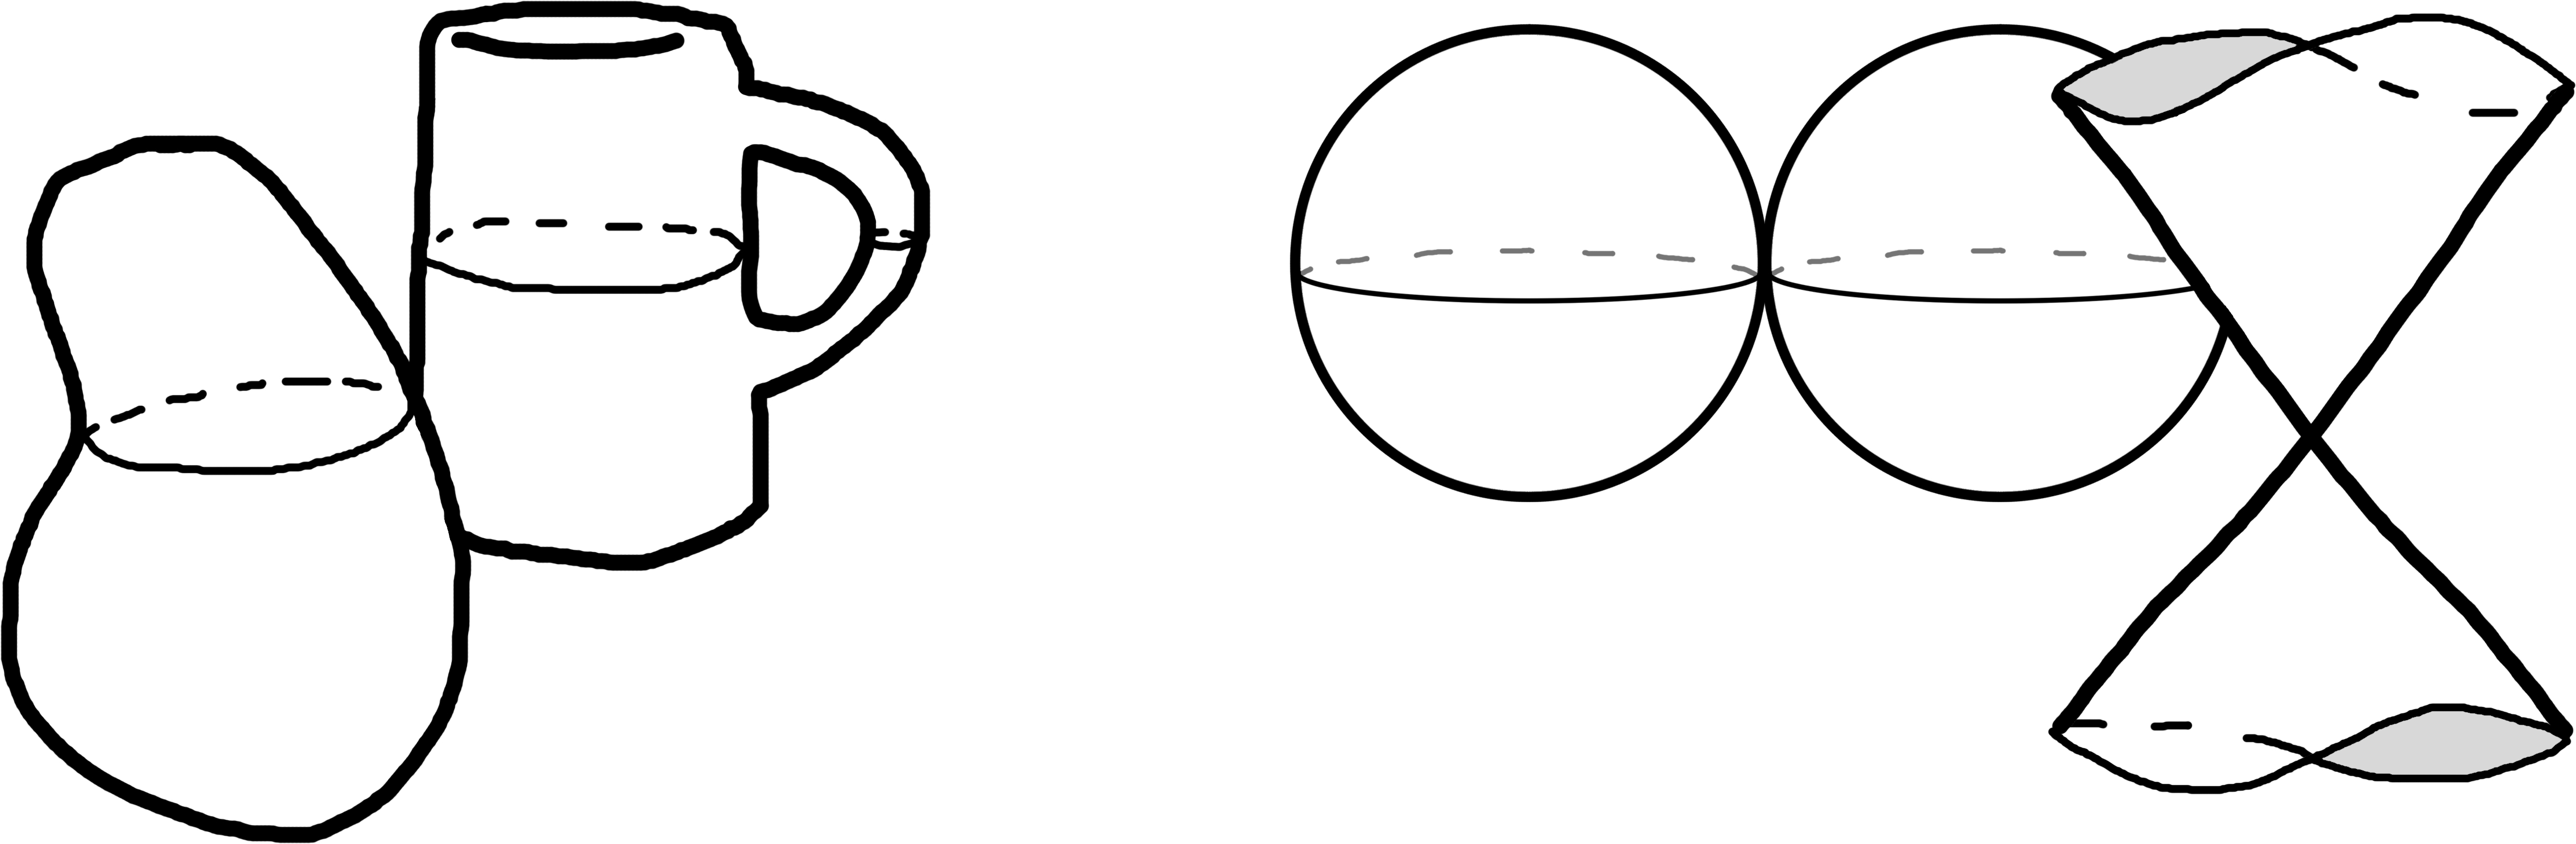
\includegraphics[scale=0.06]{maninotmani}\\
Manifolds ~~~~~~~~~~~~~~~~~~~~~~~~~~~~ Not Manifolds~~
\end{center}
Because a manifold $M$ locally \emph{looks like} $\R{n}$ we can define a similar complex which we denote $\omg{*}(M)$.
\begin{center}
\begin{tikzpicture}[scale=0.8, every node/.style={scale=0.8}]
\node (ldots) at (-6,0) {$\cdots$};
\node (C0) at (-4,0) {$\omg{k-1}(M)$};
\node (C1) at (-1.5,0) {$\omg{k}(M)$};
\node (C2) at (1,0) {$\omg{k+1}(M)$};
\node (C3) at (3.5,0) {$\omg{k+2}(M)$};
\node (rdots) at (5.5,0) {$\cdots$};

\draw
	(ldots) edge[->] (C0)
	(C0) edge[->] node[auto]{$d$} (C1)
	(C1) edge[->] node[auto]{$d$} (C2)
	(C2) edge[->] node[auto]{$d$} (C3)
	(C3) edge[->] (rdots)
;
\end{tikzpicture}
\end{center}
\end{frame}


\begin{frame}{Manifolds}
Often we're interested in studying \emph{manifolds}.
\begin{center}
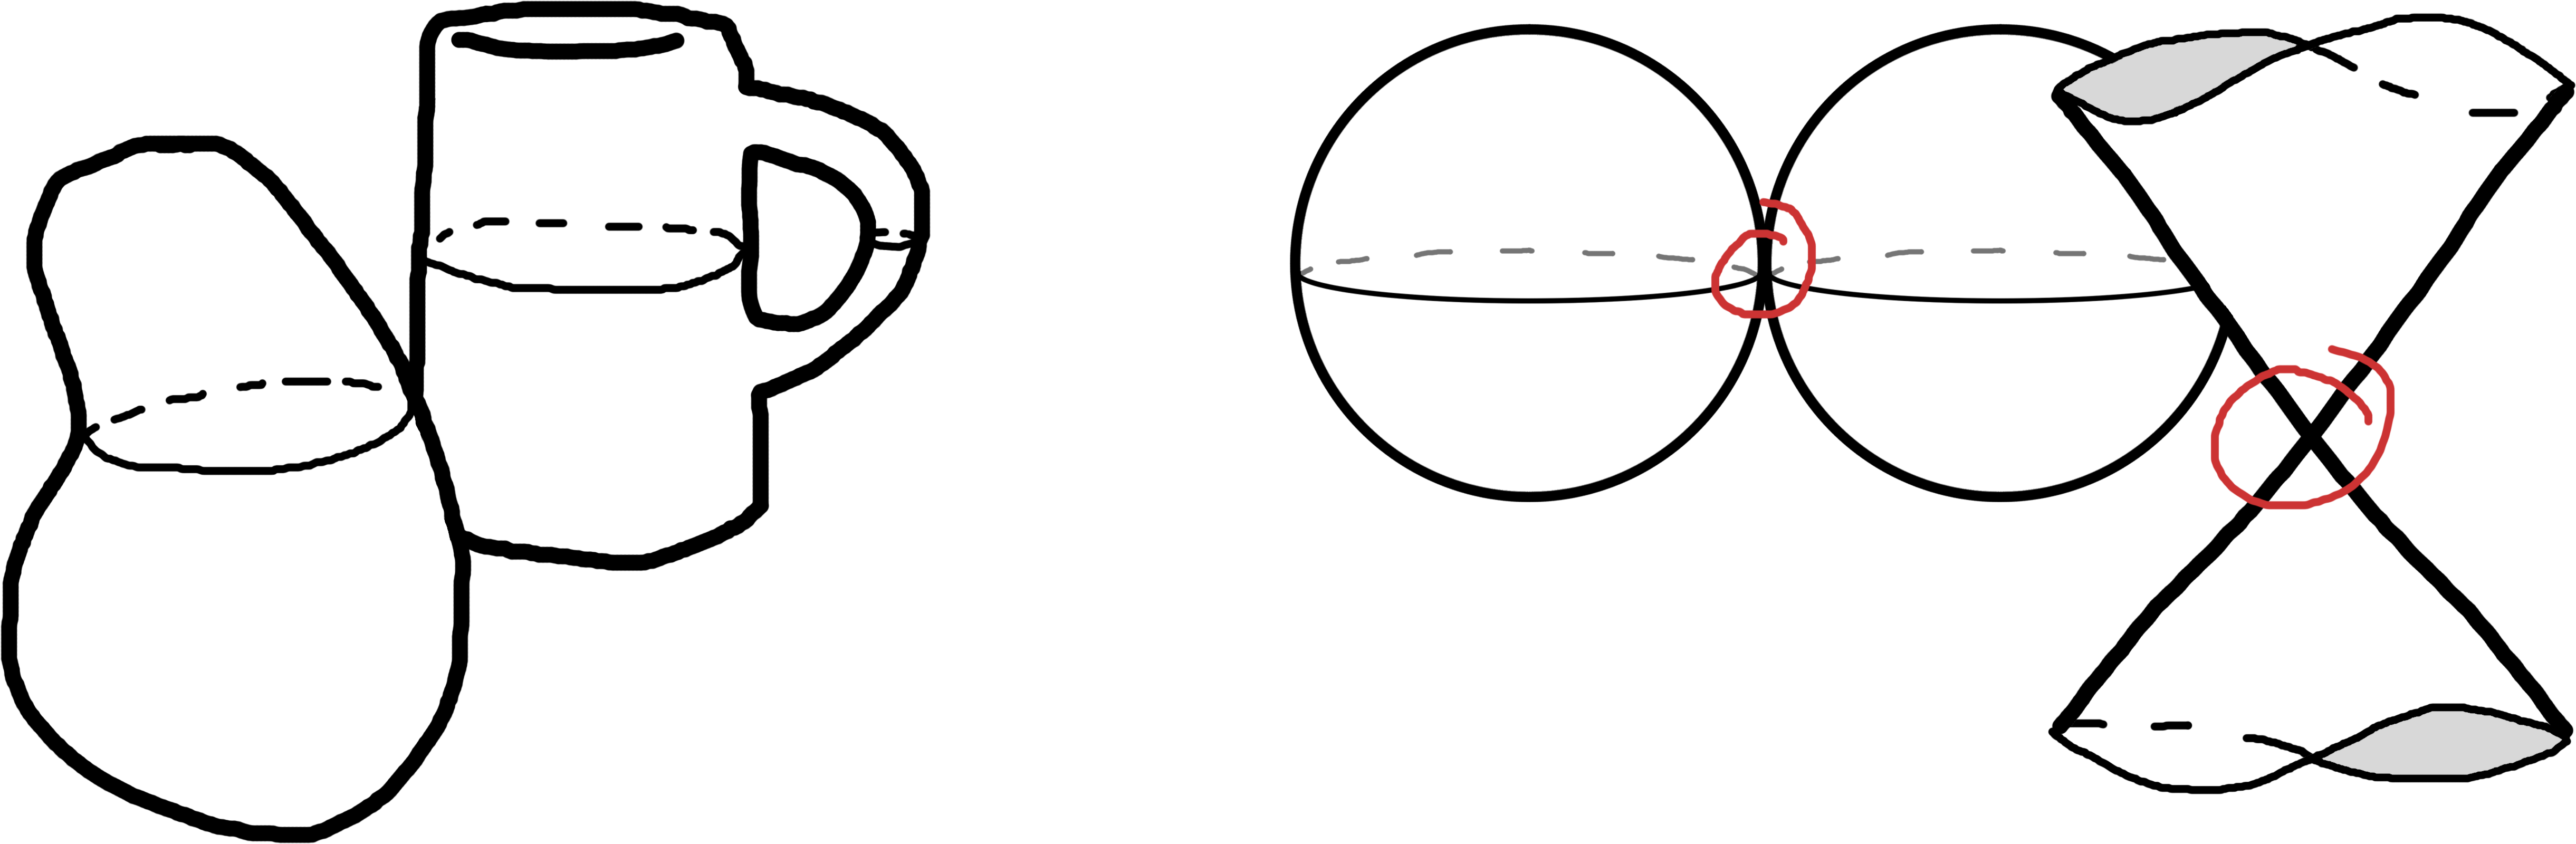
\includegraphics[scale=0.06]{maninotmaniTHERE}\\
Manifolds ~~~~~~~~~~~~~~~~~~~~~~~~~~~~ Not Manifolds~~
\end{center}
Because a manifold $M$ \emph{locally looks like} $\R{n}$ we can define a similar complex which we denote $\omg{*}(M)$.
\begin{center}
\begin{tikzpicture}[scale=0.8, every node/.style={scale=0.8}]
\node (ldots) at (-6,0) {$\cdots$};
\node (C0) at (-4,0) {$\omg{k-1}(M)$};
\node (C1) at (-1.5,0) {$\omg{k}(M)$};
\node (C2) at (1,0) {$\omg{k+1}(M)$};
\node (C3) at (3.5,0) {$\omg{k+2}(M)$};
\node (rdots) at (5.5,0) {$\cdots$};

\draw
	(ldots) edge[->] (C0)
	(C0) edge[->] node[auto]{$d$} (C1)
	(C1) edge[->] node[auto]{$d$} (C2)
	(C2) edge[->] node[auto]{$d$} (C3)
	(C3) edge[->] (rdots)
;
\end{tikzpicture}
\end{center}
\end{frame}



\begin{frame}{de Rham's Theorem}

\begin{center}
\begin{tikzpicture}[scale=0.8, every node/.style={scale=0.8}]
\node (ldots) at (-6,0) {$\cdots$};
\node (C0) at (-4,0) {$\omg{k-1}(M)$};
\node (C1) at (-1.5,0) {$\omg{k}(M)$};
\node (C2) at (1,0) {$\omg{k+1}(M)$};
\node (C3) at (3.5,0) {$\omg{k+2}(M)$};
\node (rdots) at (5.5,0) {$\cdots$};

\draw
	(ldots) edge[->] (C0)
	(C0) edge[->] node[auto]{$d$} (C1)
	(C1) edge[->] node[auto]{$d$} (C2)
	(C2) edge[->] node[auto]{$d$} (C3)
	(C3) edge[->] (rdots)
;
\end{tikzpicture}
\end{center}

From the de Rham complex of a manifold $M$, $\omg{*}(M)$, we can also define the cohomology groups analogously
\begin{align*}
H_{dR}^{q}(M)=\frac{\ker(d:\omg{q}(M) \to \omg{q+1}(M))}{\im(d:\omg{q-1}(M) \to \omg{q}(M))}
\end{align*}
for which we have the classical theorem of de Rham's.
\begin{block}{de Rham's Theorem}
Let $M$ be a smooth manifold. Then there is an isomorphism
\[
H_{dR}^{*}(M) \cong H^{*}(M).
\]
\end{block}
\end{frame}



\begin{frame}{Group action on a manifold}
Sometimes we're interested in studying a group $G$ \emph{acting} on a manifold $M$.
\begin{center}
\includegraphics[scale=0.04]{"Group action sphere"}
\end{center}
\begin{block}{Question:}
Can we define a cohomology theory for $M$ that reflects the geometry of $M$ \emph{and} the action of the group $G$?
\end{block}
Let $M/G$ denote the orbit space -- that is, impose the relation $x \sim y \iff x= y \cdot g$ for some $g\in G$. What does the cohomology of $M/G$ tell us?
\end{frame}



\begin{frame}{Naive approach}
Answer: Not much.
\begin{exampleblock}{Calculating $H^{*}(S^{2}/S^{1})$}
\begin{center}
\includegraphics[scale=0.04]{"quotient"}
\end{center}
The quotient of the sphere by the circle is isomorphic to the interval $[-1,1]$ which is homotopy equivalent to a point.
\[
S^{2}/S^{1} \simeq [-1,1] \simeq \{\mathrm{pt}\}.
\]
Thus, $H^{*}(S^{2}/S^{1})$ is trivial.
\end{exampleblock}
Where are we losing so much information?
\end{frame}


\begin{frame}{Naive approach}
%I'll try to explain where we are losing information in less than 6 seasons
One problem is that the group $G$ is not acting \emph{freely} on the manifold $M$ and so the quotient $M/G$ is losing too much information.
\begin{center}
\includegraphics[scale=0.04]{"quotient2"}
\end{center}
\begin{block}{Free action of a group on a manifold}
Let $G$ be a group acting on a topological space $X$. We say that the action of $G$ is \emph{free} if, for every $x \in X$
\[
x \cdot g = x \iff g \text{ is the identity}.
\]
\end{block}
\end{frame}



\begin{frame}{What should we do?}
\begin{block}{Proposition}
 Let $X$ and $Y$ be $G$-sets such that $G$ acts freely on $X$. Then $G$ acts freely on $X \times Y$.
\end{block}
Solution: Find a {\color<3->{red} suitable space $E$} on which $G$ acts freely and calculate the cohomology of the orbit space of the product
\[
H^{*}((M\times E)/G).
\]
\visible<2->{More problems:}
\begin{enumerate}
\item<3-> What is $E$?
\item<4-> Is this still related to the original problem?
\item<5-> Is this an easy calculation?
\end{enumerate}
\end{frame}

\begin{frame}{A suitable space}
There \emph{is} a \emph{topological space}, $EG$, for every group $G$ such that 
\begin{itemize}
\item $G$ acts freely on $EG$.
\item $EG$ is contractible
\end{itemize}
\uncover<2->{
If $M$ is a manifold with group action $G$,
\begin{itemize}
\item $G$ is free on $M \times EG$
\item $M$ is homotopy equivalent to $M \times EG$
\end{itemize}
}
\uncover<3->{
It is also possible to show that, for any topological space $X$ with $G$-action and contractible space $E$ on which $G$ acts freely, the cohomology group
\[
H^{*}((X \times E)/G)
\]
is independent of the choice of E.
}
\end{frame}



\begin{frame}{We have a model}
We will define the \emph{homotopy quotient}
\[
M // G := (M \times EG) / G
\]
and define the \emph{equivariant cohomology} of a manifold $M$ by
\[
H^{*}_G(M) := H^{*}(M // G).
\]
\end{frame}



\begin{frame}{Equivariant de Rham theory}
\begin{block}{Question:}
Can we come up with an analogue of de Rham's theorem for equivariant cohomology? 
\end{block}
To be able to form a de Rham complex on $M//G$,
\[
\omg{*}(M//G),
\]
 we would require $(M \times EG)/G$ to be a manifold. Instead we can look at the \emph{``Cartan model"}
 \[
 \omg{*}_G(M)
 \]
 which is an \emph{equivariant version} of the de Rham complex.
\end{frame}



\begin{frame}{Equivariant de Rham theory}
\begin{block}{Question:}
Can we come up with an analogue of de Rham's theorem for equivariant cohomology? 
\end{block}
To be able to form a de Rham complex on $M//G$,
\[
\omg{*}(M//G),
\]
 we would require $(M \times EG)/G$ to be a manifold. Instead we can look at the \emph{``Cartan model"}
 \[
 \omg{*}_G(M)=(\omg{*}(M) \otimes S^*(\mathfrak{g}^*))^G
 \]
 which is an \emph{equivariant version} of the de Rham complex.
\end{frame}



\begin{frame}{A classical theorem}
From the Cartan Model we have the following theorem:
\begin{block}{Equivariant de Rham theorem}
Let $G$ be a compact, connected Lie group and $M$ be a manifold with $G$-action. Then there is an isomorphism
\[
H^{*}_G(M) \cong H^{*}(\omg{*}_G(M)).
\]
\end{block}
\begin{alertblock}{Goal}
The goal of my project will be to realise this isomorphism explicitly using simplicial methods.
\end{alertblock}
\end{frame}



\begin{frame}{Simplicial Methods}

The action of a Lie group on a manifold can also be captured in a \emph{simplicial manifold}, $M_{\bullet}$. Consider the sequence of manifolds
\begin{center}
	\begin{tikzpicture}
	%Nodes
	\node (M0) at (0,0) {$M$};
	\node (M1) at (3,0) {$M \times G$};
	\node (M2) at (6.5,0) {$M \times G \times G$};
	\node (D) at (10.4,0) {$\cdots$};
	%Left arrows
	\draw
		(2.3,0.15) edge[->] node[above]{$d_0, d_1$} (0.35,0.15)
		(2.3,0.05) edge[->] (0.35,0.05)
		
		(5.5,0.25) edge[->] node[above]{$d_0, d_1, d_2$} (3.65,0.25)
		(5.5,0.15) edge[->] (3.65,0.15)
		(5.5,0.05) edge[->] (3.65,0.05)
		
		(10,0.35) edge[->] node[above]{$d_0, d_1, d_2,d_3$} (7.65,0.35)
		(10,0.25) edge[->] (7.65,0.25)
		(10,0.15) edge[->] (7.65,0.15)
		(10,0.05) edge[->] (7.65,0.05)
	;
	%Right arrows
	\draw
		(0.35,-0.15) edge[->] node[below]{$s_0$} (2.3,-0.15)
		
		(3.65,-0.15) edge[->] (5.5,-0.15)
		(3.65,-0.25) edge[->] node[below]{$s_0, s_1$} (5.5,-0.25)
		
		(7.65,-0.15) edge[->] (10,-0.15)
		(7.65,-0.25) edge[->] (10,-0.25)
		(7.65,-0.35) edge[->] node[below]{$s_0, s_1,s_2$} (10,-0.35)
	;
	\end{tikzpicture}
\end{center}
with \emph{face} and \emph{degeneracy} maps, $d_i$ and $s_j$ respectively. We will form a cohomology theory for this \emph{simplicial manifold} that computes the equivariant cohomology of $M$ with $G$-action.
\end{frame}


\begin{frame}{A simplex}
%%%%%%%%%%%%%%%%%%%%%%%%%%%%%%%%%%%%%%%%%%%%%%%%
%%%   MAKE SURE TO MENTION ON THIS SLIDE THAT Delta^n IS A MANIFOLD TOO!!!   %%%
%%%%%%%%%%%%%%%%%%%%%%%%%%%%%%%%%%%%%%%%%%%%%%%%
The standard topological \emph{$n$-simplex} is the set of points
\[
\Delta^n = \{(t_0,t_1,\cdots,t_n)\in\R{n+1}: \: t_0+t_1+\cdots+t_n = 1, t_i \geq 0 \}.
\]
This topological space is special because we can decompose the boundary of $\Delta^n$ into components that are homeomorphic to $\Delta^{n-1}$. Another way to think about this is that there are \emph{canonical inclusions and projections}
\[
d^i:\Delta^n \to \Delta^{n+1}, \: s^i:\Delta^n \to \Delta^{n-1}.
\]
\begin{center}
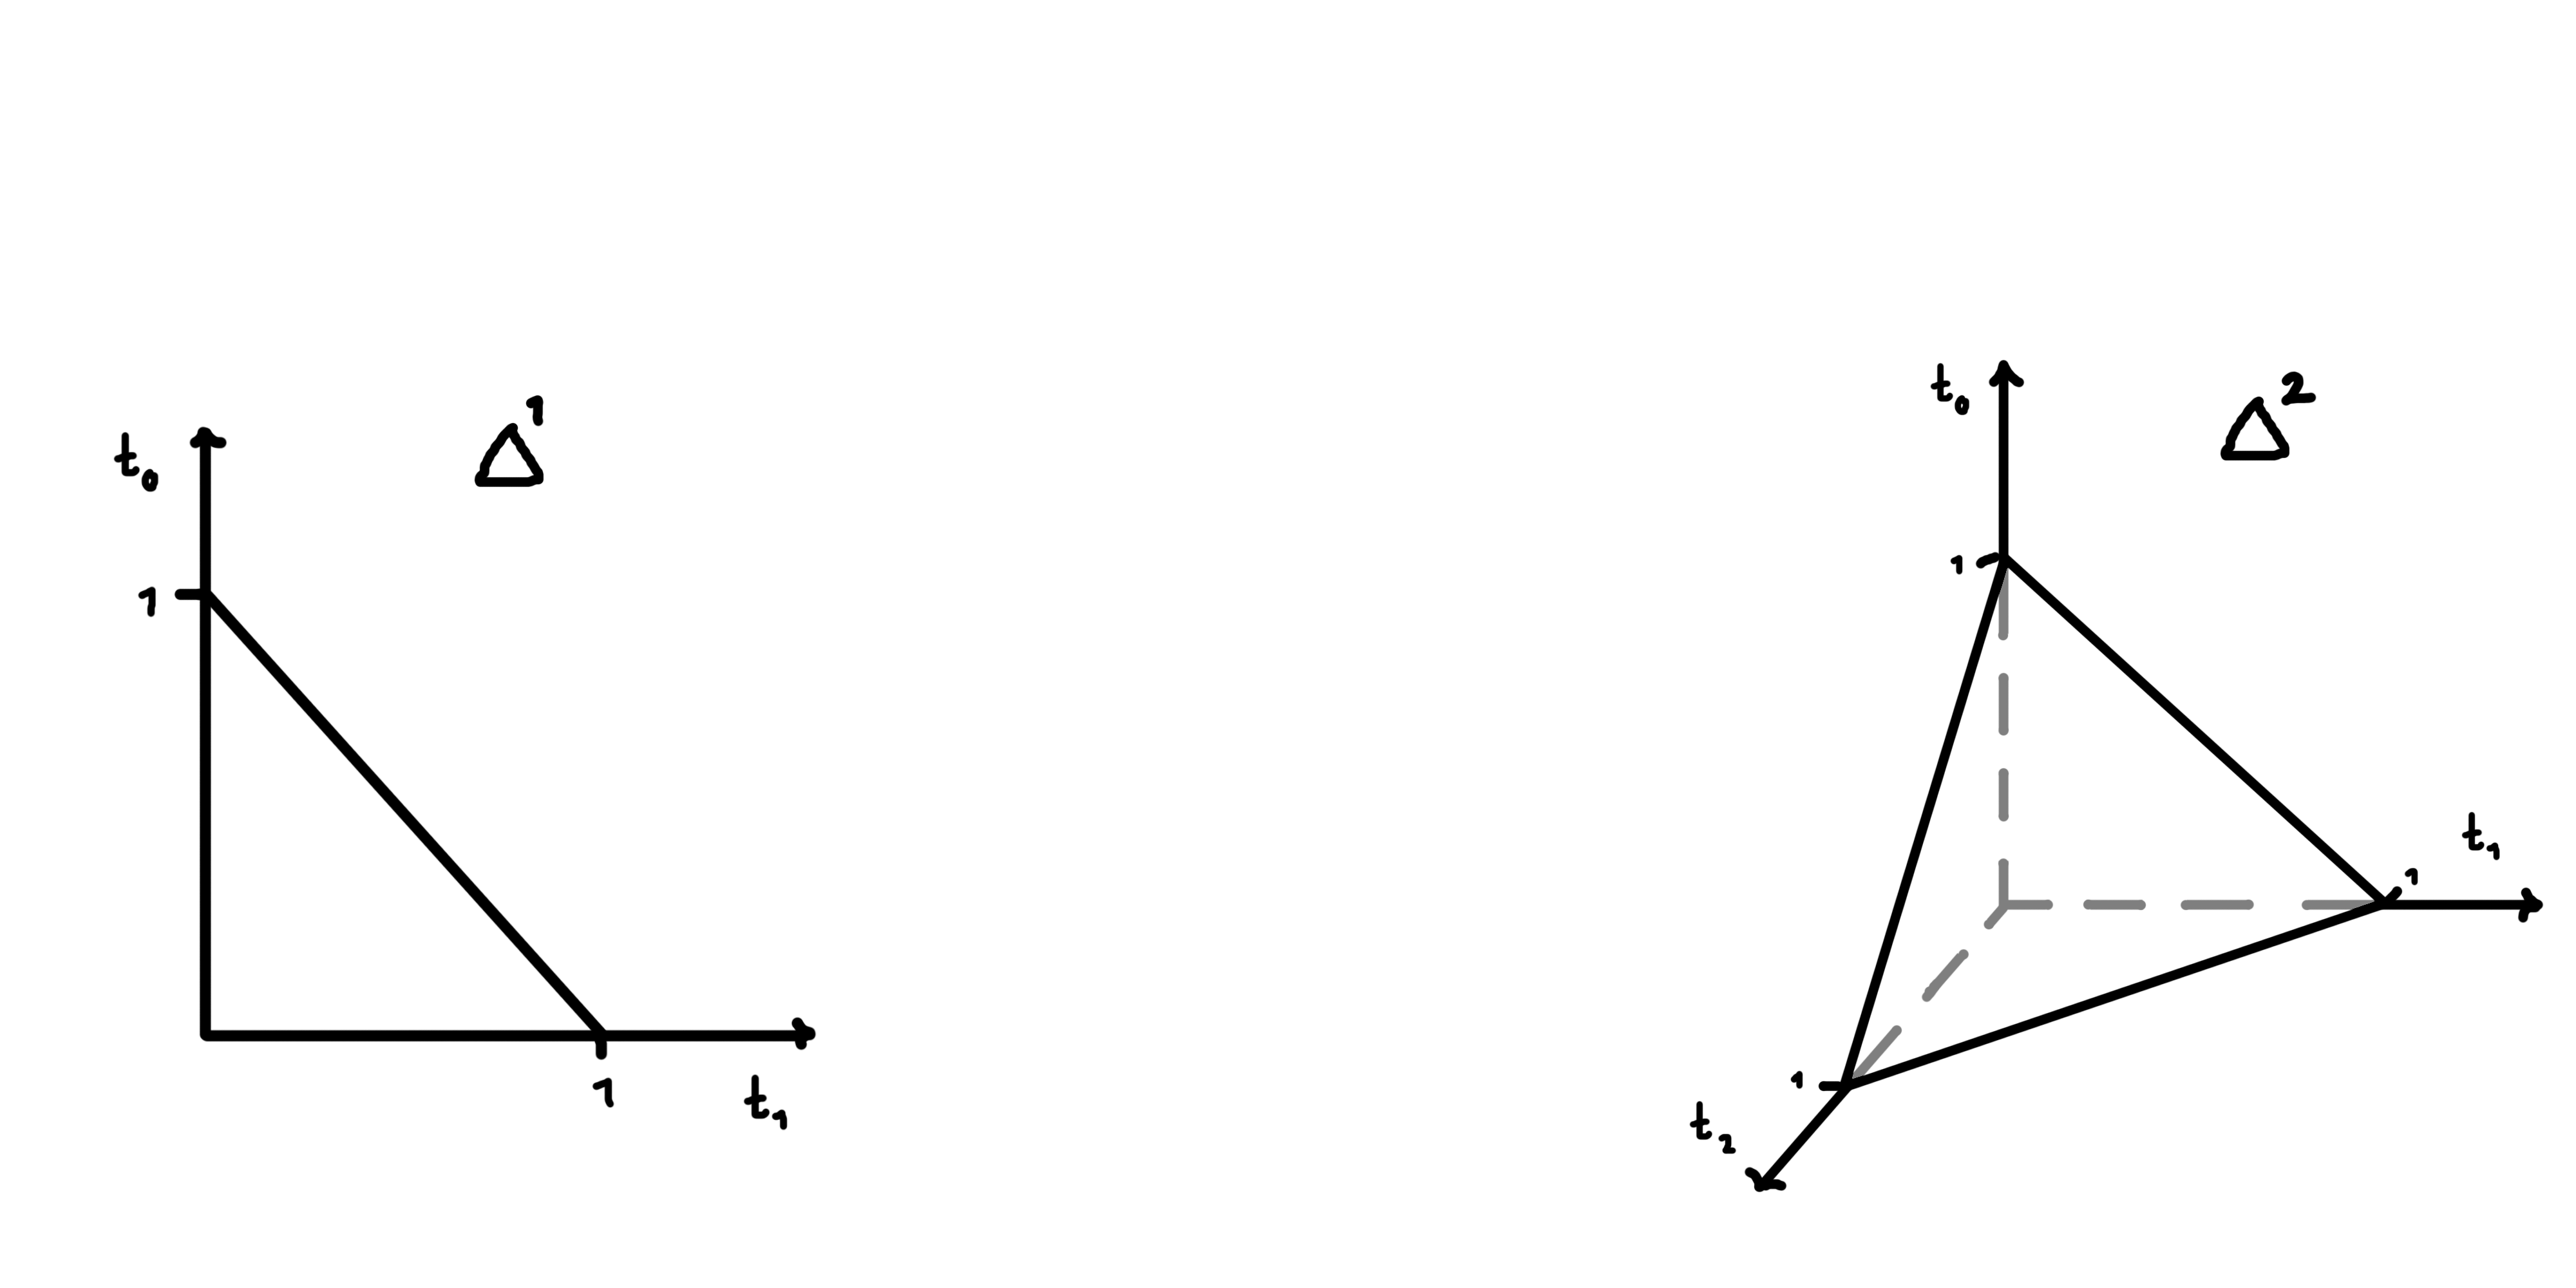
\includegraphics[scale=0.06]{simplicies}
\end{center}
%We use simplicial methods to build a sequence of spaces that have similar relationships encoded into them.
\end{frame}



\begin{frame}{A simplex}
%%%%%%%%%%%%%%%%%%%%%%%%%%%%%%%%%%%%%%%%%%%%%%%%
%%%   MAKE SURE TO MENTION ON THIS SLIDE THAT Delta^n IS A MANIFOLD TOO!!!   %%%
%%%%%%%%%%%%%%%%%%%%%%%%%%%%%%%%%%%%%%%%%%%%%%%%
The standard topological \emph{$n$-simplex} is the set of points
\[
\Delta^n = \{(t_0,t_1,\cdots,t_n)\in\R{n+1}: \: t_0+t_1+\cdots+t_n = 1, t_i \geq 0 \}.
\]
This topological space is special because we can decompose the boundary of $\Delta^n$ into components that are homeomorphic to $\Delta^{n-1}$. Another way to think about this is that there are \emph{canonical inclusions and projections}
\[
d^i:\Delta^n \to \Delta^{n+1}, \: s^i:\Delta^n \to \Delta^{n-1}.
\]
\begin{center}
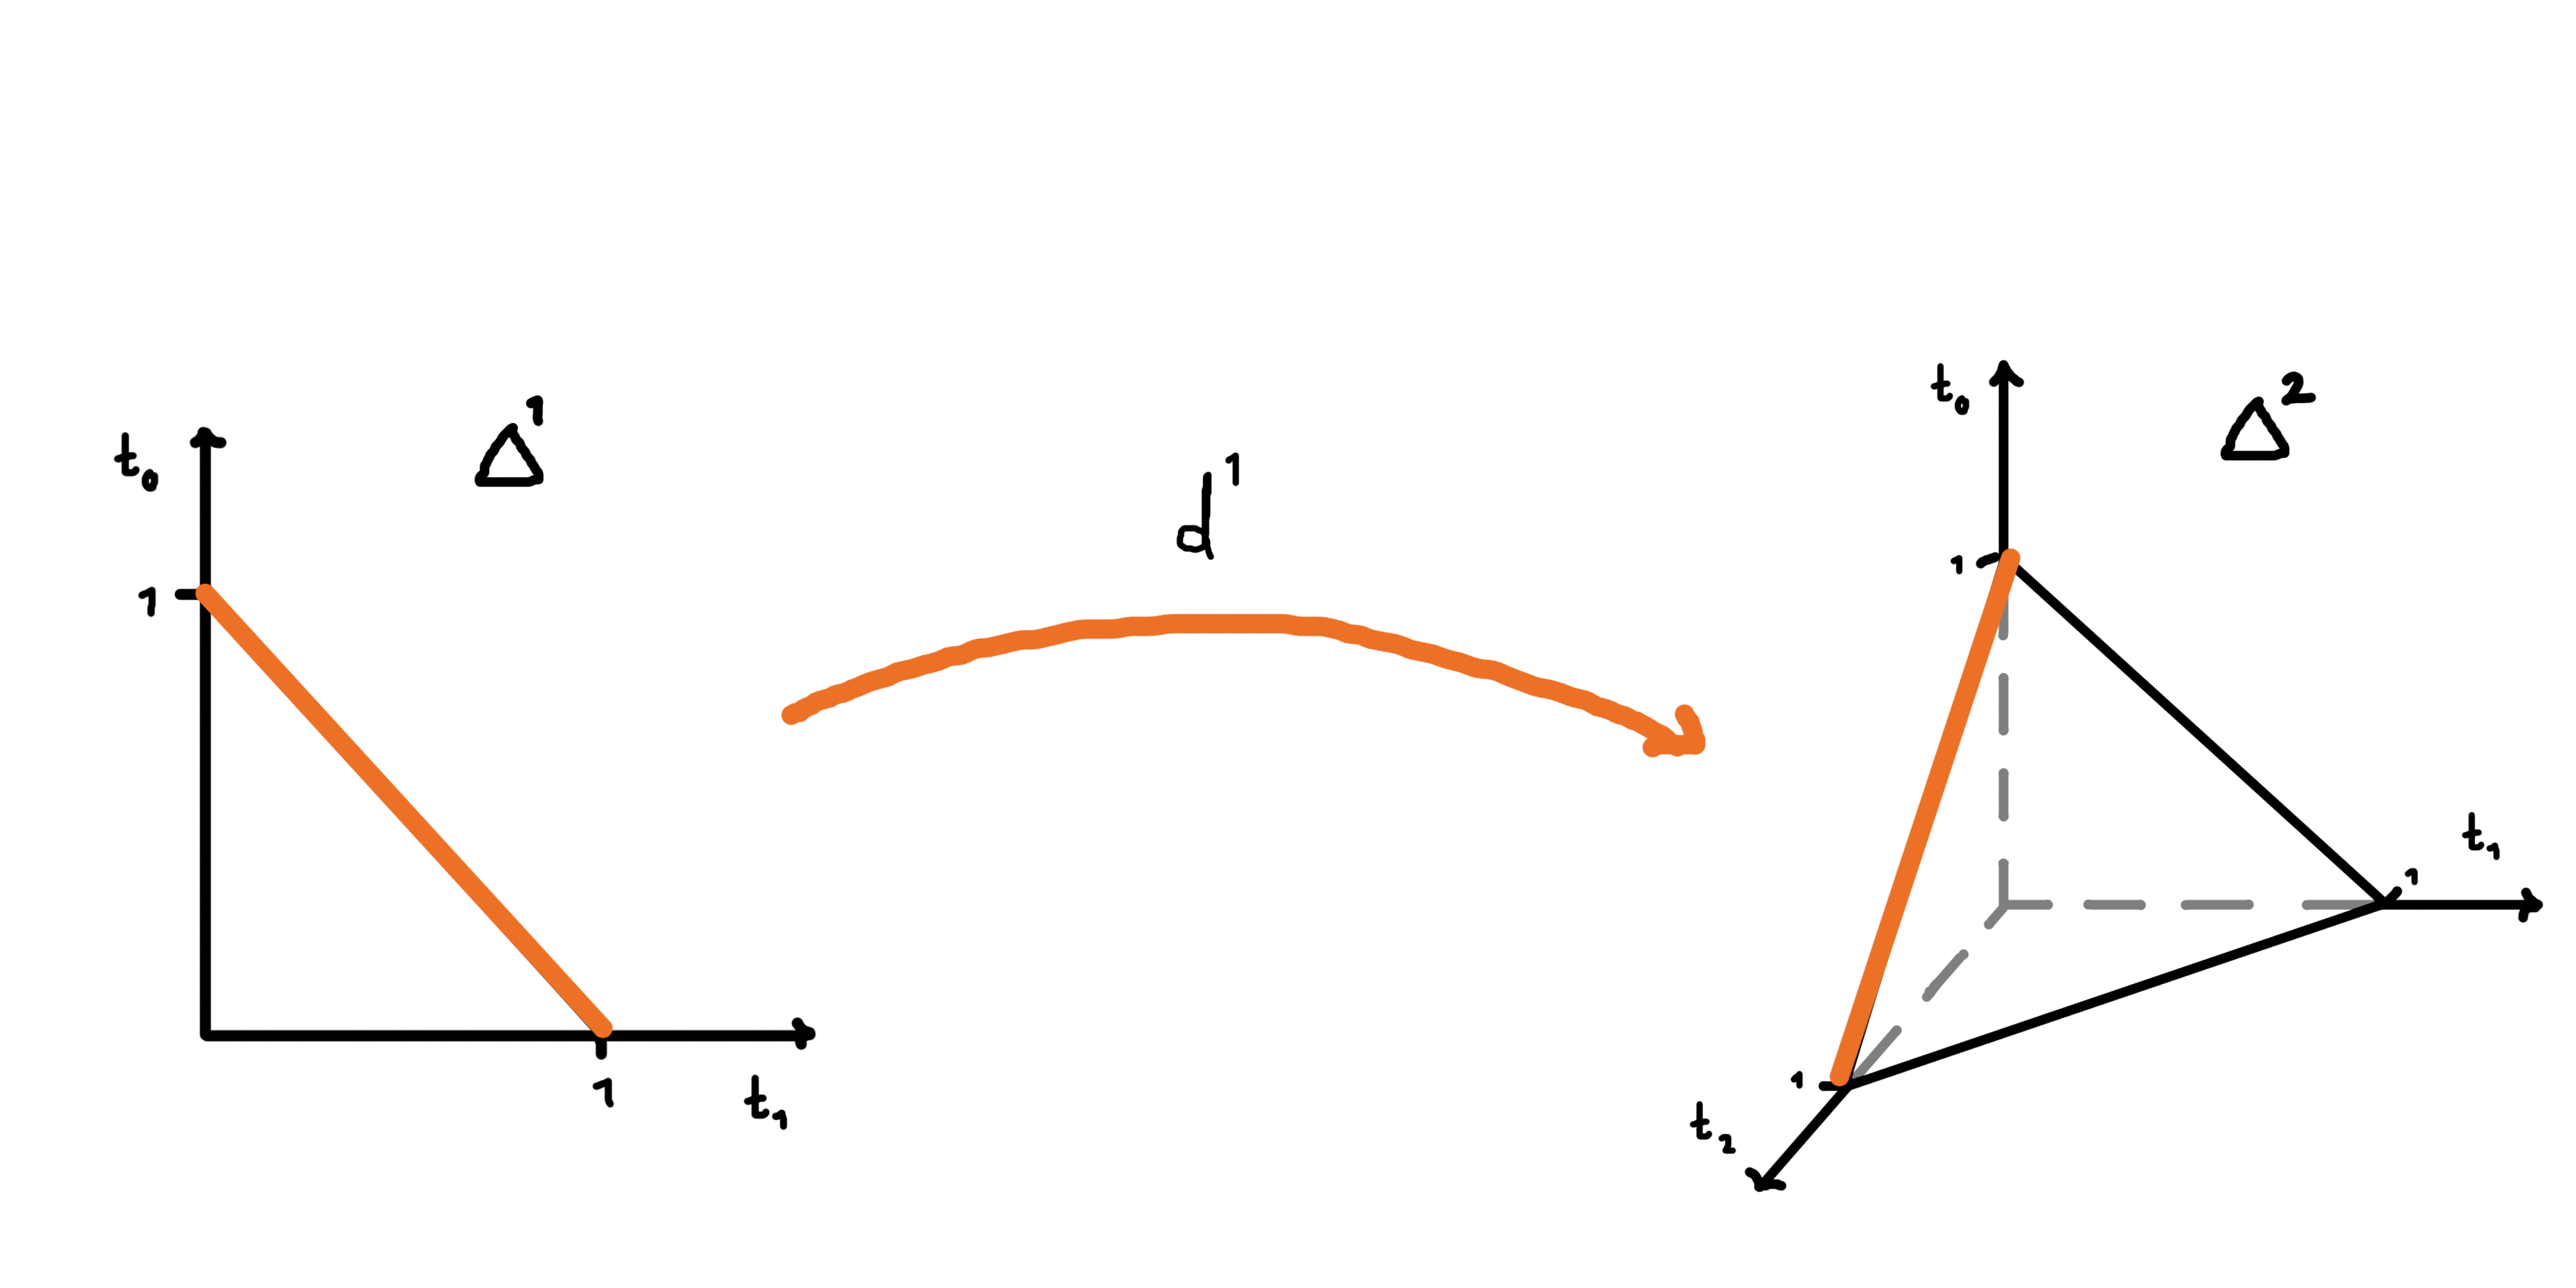
\includegraphics[scale=0.06]{simpliciesupmap}
\end{center}
%We use simplicial methods to build a sequence of spaces that have similar relationships encoded into them.
\end{frame}



\begin{frame}{Simplicial Manifolds}

Let $X_{\bullet} = \{X_q\}_{q\geq0}$ be a sequence of manifolds
\begin{center}
	\begin{tikzpicture}
	%Nodes
	\node (M0) at (0,0) {$X_0$};
	\node (M1) at (2.5,0) {$X_1$};
	\node (M2) at (5,0) {$X_2$};
	\node (D) at (7.5,0) {$\cdots$};
	%Left arrows
	\draw
		(2.2,0.15) edge[->] node[above]{$d_0, d_1$} (0.25,0.15)
		(2.2,0.05) edge[->] (0.25,0.05)
		
		(4.7,0.25) edge[->] node[above]{$d_0, d_1,d_2$} (2.75,0.25)
		(4.7,0.15) edge[->] (2.75,0.15)
		(4.7,0.05) edge[->] (2.75,0.05)
		
		(7.1,0.35) edge[->] node[above]{$d_0, d_1, d_2,d_3$} (5.25,0.35)
		(7.1,0.25) edge[->] (5.25,0.25)
		(7.1,0.15) edge[->] (5.25,0.15)
		(7.1,0.05) edge[->] (5.25,0.05)
	;
	%Right arrows
	\draw
		(0.25,-0.15) edge[->] node[below]{$s_0$} (2.2,-0.15)
		
		(2.75,-0.15) edge[->] (4.7,-0.15)
		(2.75,-0.25) edge[->] node[below]{$s_0, s_1$} (4.7,-0.25)
		
		(5.25,-0.15) edge[->] (7.1,-0.15)
		(5.25,-0.25) edge[->] (7.1,-0.25)
		(5.25,-0.35) edge[->] node[below]{$s_0, s_1,s_2$} (7.1,-0.35)
	;
	\end{tikzpicture}
\end{center}
with \emph{face} and \emph{degeneracy} maps, $d_i$ and $s_j$ respectively. We call $X_{\bullet}$ a simplicial manifold if the face and degeneracy maps are smooth and satisfy
\begin{itemize}
\item $d_i \, d_j = d_{j-1} \, d_i$ if $i < j$
\item $s_i \, s_j = s_{j+1} \, s_i$ if $i \leq j$
\item $d_i \, s_j = \left\{ \begin{array}{ll}
					   s_{j-1} \, d_i  & \mbox{if } i<j \\
					   ~~~\mbox{id}_{X_i}  & \mbox{if } i=j, i=j+1\\
					   s_j \, d_{i-1} & \mbox{if } i > j+1
					   \end{array}
					   \right.$
\end{itemize}
\end{frame}



\begin{frame}{Simplicial Methods}
Let's look again at the simplicial manifold we are interested in. In particular, we want to define the maps
\[
M \times G^{n-1} \xleftarrow{\mathmakebox[1cm]{d_i}} M \times G^{n} \xrightarrow{\mathmakebox[1cm]{s_i}} M \times G^{n+1}.
\]
for $0 \leq i \leq n$ where $M \times G^n = M \times G \times G \times \cdots \times G$.
An element of $M \times G^n$ will be of the form
\[
(m, g_0, g_1, \cdots, g_{n-1}), ~~~~ m \in M,\ g_i \in G
\]
so we could define the maps $d_i$ and $s_i$ by
\begin{align*}
d_i(m, g_0, \cdots, g_{n-1}) &= (m, g_0, \cdots, g_{i-2}, g_{i-1} \cdot g_i, g_{i+1}, \cdots, g_{n-1})\\
s_i(m, g_0, \cdots, g_{n-1}) &= (m, g_0, \cdots, g_{i-1}, 1, g_{i}, \cdots, g_{n-1})
\end{align*}
to form a simplicial manifold.
\end{frame}

\begin{frame}{Geometric Realisation}
Encoded into the simplicial manifold $M_{\bullet}$ is precisely the group action of $G$ on the manifold $M$.
\[
d_0(m,g) = m \cdot g
\]
We can stick all this information into a single topological space which we call the \emph{geometric realisation} $|M_{\bullet}|$ which leaves us with a familiar topological space.
\[
|M_{\bullet}| ~ = ~ \coprod\limits_{n\geq0} \Delta^{n} \times M \times G^{n} / \sim ~ = ~ M // G
\]
This means if we can form a de Rham theory for the simplicial manifold $M_{\bullet}$ we may be able to relate it back to the equivariant cohomology of $M$ with $G$-action.
\end{frame}



\begin{frame}{Simplicial de Rham complex}
Since $G$ is a Lie group, each of the spaces $M \times G^{n}$ is a manifold. This means that we can form de Rham complexes of differential forms
\[
\omg{*}(M \times G^{n}).
\]
The smooth face maps, $d_i : M \times G^{n} \to M \times G^{n-1}$ induce pullback maps
\[
d_i^* : \omg{*}(M \times G^{n-1}) \to \omg{*}(M \times G^{n}).
\]
From this we can construct a complex
\begin{center}
\begin{tikzpicture}[scale=0.8, every node/.style={scale=0.8}]
\node (ldots) at (-6,0) {$\cdots$};
\node (C0) at (-3.5,0) {$\omg{k}(M \times G^{n-1})$};
\node (C1) at (0,0) {$\omg{k}(M \times G^{n})$};
\node (C2) at (3.5,0) {$\omg{k}(M \times G^{n+1})$};
\node (rdots) at (6,0) {$\cdots$};

\draw
	(ldots) edge[->] (C0)
	(C0) edge[->] node[auto]{$\delta$} (C1)
	(C1) edge[->] node[auto]{$\delta$} (C2)
	(C2) edge[->] (rdots)
;
\end{tikzpicture}
\end{center}
where $\delta: \omg{*}(M \times G^{n-1}) \to \omg{*}(M \times G^{n})$ is defined to be
\[
\delta = \sum\limits_{i=0}^{n} (-1)^{i}d_i^*.
\]
\end{frame}



\begin{frame}{Double complex}
Because we have two differential operators defined on $\omg{p}(M \times G^{q})$, we can form a double complex.
\begin{center}
	\begin{tikzpicture}[every node/.style={scale=0.8}]
		\node (00) at (0,0) {$\omg{0}(M)$};
		\node (01) at (0,2) {$\omg{1}(M)$};
		\node (02) at (0,4) {$\omg{2}(M)$};
		\node (03) at (0,5.5) {$\vdots$};
		\node (10) at (2,0) {$\omg{0}(M \times G)$};
		\node (11) at (2,2) {$\omg{1}(M \times G)$};
		\node (12) at (2,4) {$\omg{2}(M \times G)$};
		\node (13) at (2,5.5) {$\vdots$};
		\node (20) at (4.5,0) {$\omg{0}(M \times G^2)$};
		\node (21) at (4.5,2) {$\omg{1}(M \times G^2)$};
		\node (22) at (4.5,4) {$\omg{2}(M \times G^2)$};
		\node (23) at (4.5,5.5) {$\vdots$};
		\node (30) at (7,0) {$\omg{0}(M \times G^3)$};
		\node (31) at (7,2) {$\omg{1}(M \times G^3)$};
		\node (32) at (7,4) {$\omg{2}(M \times G^3)$};
		\node (33) at (7,5.5) {$\vdots$};
		\node (40) at (9,0) {$\cdots$};
		\node (41) at (9,2) {$\cdots$};
		\node (42) at (9,4) {$\cdots$};
		%
		\draw[->]
			%Vertical arrows
			(00) edge node[auto]{$d$} (01)
			(01) edge node[auto]{$d$} (02)
			(02) edge (03)
			
			(10) edge node[auto]{$d$} (11)
			(11) edge node[auto]{$d$} (12)
			(12) edge (13)
			
			(20) edge node[auto]{$d$} (21)
			(21) edge node[auto]{$d$} (22)
			(22) edge (23)
			
			(30) edge node[auto]{$d$} (31)
			(31) edge node[auto]{$d$} (32)
			(32) edge (33)
			
			%Horizontal arrows
			(00) edge node[auto]{$\delta$} (10)
			(10) edge node[auto]{$\delta$} (20)
			(20) edge node[auto]{$\delta$} (30)
			(30) edge (40)
			
			(01) edge node[auto]{$\delta$} (11)
			(11) edge node[auto]{$\delta$} (21)
			(21) edge node[auto]{$\delta$} (31)
			(31) edge (41)
			
			(02) edge node[auto]{$\delta$} (12)
			(12) edge node[auto]{$\delta$} (22)
			(22) edge node[auto]{$\delta$} (32)
			(32) edge (42)
		;
		
	\end{tikzpicture}
\end{center}
\end{frame}



\begin{frame}{Total complex}
We want to pull a cohomology theory out of this double complex, so we are going to try to reduce this to a regular complex.
\begin{center}
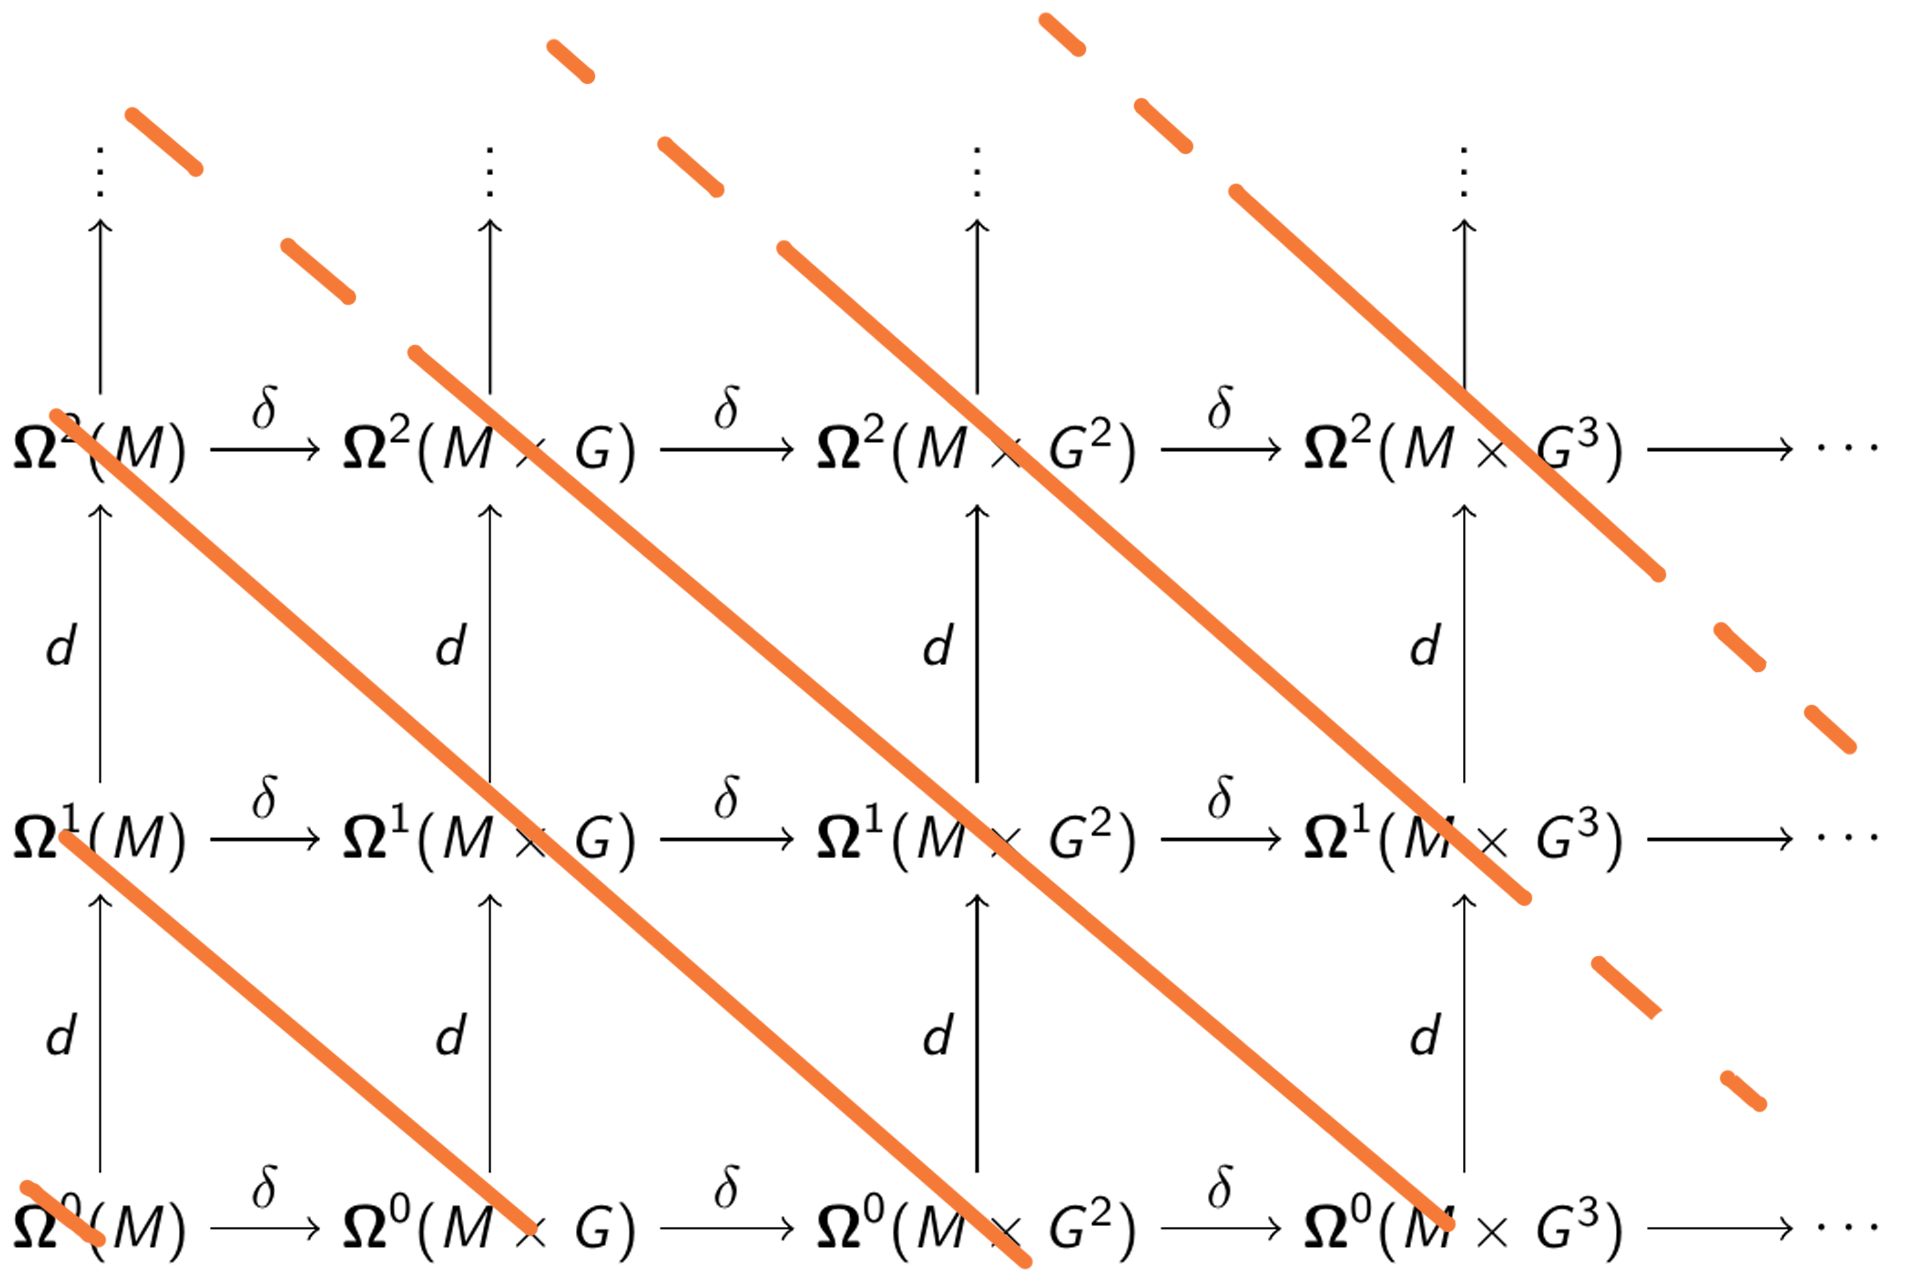
\includegraphics[scale=0.12]{totalcomplex}
\end{center}
\begin{center}
\begin{tikzpicture}[scale=0.5, every node/.style={scale=0.5}]
\node (C0) at (-7,0) {$\omg{0}(M\times G^0)$};
\node (C1) at (-3,0) {$\bigoplus\limits_{p+q=1}\omg{p}(M\times G^q)$};
\node (C2) at (2,0) {$\bigoplus\limits_{p+q=2}\omg{p}(M\times G^q)$};
\node (C3) at (6.5,0) {$\bigoplus\limits_{p+q=3}\omg{p}(M\times G^q)$};
\node (rdots) at (10,0) {$\cdots$};

\draw
	(C0) edge[->] (C1)
	(C1) edge[->] (C2)
	(C2) edge[->] (C3)
	(C3) edge[->] (rdots)
;
\end{tikzpicture}
\end{center}


\end{frame}



\begin{frame}{Total complex}

\begin{center}
\begin{tikzpicture}[scale=0.75, every node/.style={scale=0.75}]
\node (ldots) at (-7.5,0) {$\cdots$};
\node (C0) at (-5,0) {$\bigoplus\limits_{p+q=n-1}\omg{p}(M\times G^q)$};
\node (C1) at (0,0) {$\bigoplus\limits_{p+q=n}\omg{p}(M\times G^q)$};
\node (C2) at (5,0) {$\bigoplus\limits_{p+q=n+1}\omg{p}(M\times G^q)$};
\node (rdots) at (7.5,0) {$\cdots$};

\draw
	(ldots) edge[->] (C0)
	(C0) edge[->] node[auto]{$D$} (C1)
	(C1) edge[->] node[auto]{$D$} (C2)
	(C2) edge[->] (rdots)
;
\end{tikzpicture}
\end{center}

We can define a differential operator on this sequence
\[
D:\bigoplus\limits_{p+q=n}\omg{p}(M\times G^q) \xrightarrow{~~~~} \bigoplus\limits_{p+q=n+1}\omg{p}(M\times G^{q})
\]
defined by
\[
D = \delta + (-1)^{p}d.
\]
Since $D^2 = 0$ we can construct a new \emph{total complex} $~\omg{*}_{total}(M_{\bullet})$.

\begin{block}{Theorem}
Let $M$ be a manifold with smooth $G$-action for $G$ a compact Lie group. Then there is an isomorphism
\[
H^{*}(\omg{*}_{total}(M_{\bullet})) \cong H^{*}(|M_{\bullet}|)
\]
\end{block}
\end{frame}



\begin{frame}{An important example}
The case where we take our manifold $M$ to be a point may seem trivial after this discussion, but this is precisely the work we wish to extend. In his monograph \emph{Curvature and Characteristic Classes}, Dupont uses this model to calculate the equivariant cohomology of a point and shows that
\[
S^{*}(\mathfrak{g}^{*})^G \cong H^*(\omg{*}_{total}(\{pt\}_{\bullet})) \cong H^{*}_G(\{pt\}).
\]
By extending this work we wish to show an explicit isomorphism from the Cartan model of equivariant cohomology to the simplicial case.
\[
H^{*}(\omg{*}_{total}(M_{\bullet})) \xrightarrow{~~~\cong~~~} H^{*}((\omg{*}(M) \otimes S^{*}(\mathfrak{g}^{*}))^G)
\]
\end{frame}



\begin{frame}{Acknowledgements}
\begin{center}
I would like to take this opportunity to acknowledge and thank my supervisors Danny Stevenson and Michael Murray.
\end{center}
\end{frame}




\begin{frame}{Questions?}

\end{frame}



\begin{frame}{Extra: Geometric Realisation}

\[
|M_{\bullet}| ~ = ~ \coprod\limits_{n\geq0} \Delta^{n} \times M \times G^{n} / \sim
\]
\begin{center}
\end{center}
Where for $t \in \Delta^n$, $m \in M$ and $(g_0,\cdots,g_{n-1})\in G^{n}$ we have the identifications
\begin{itemize}
\item $(d^{i}t, (m, g_0,\cdots,g_{n-1})) \sim (t, d_i(m, g_0,\cdots,g_{n-1})$
\item $(s^{i}t, (m, g_0,\cdots,g_{n-1})) \sim (t, s_i(m, g_0,\cdots,g_{n-1}))$
\end{itemize}

\end{frame}

\begin{frame}{Extra: $D^2 = 0$}
We defined
\[
D = \delta + (-1)^p d.
\]
Note that $\delta$ is the sum of pullback maps $d_i$ and hence commutes with $d$. The task is then showing that $D^2=0$ for each element in the sum
\[
\bigoplus\limits_{p+q=n}\omg{p}(M\times G^q)
\]
\begin{align*}
D^2 &= \delta^2 + \delta(-1)^{p}d + (-1)^{p-1}d\delta + (-1)^{2p}d\\
&= 0 + \delta(-1)^{p}d + \delta(-1)^{p-1}d + 0\\
&= 0
\end{align*}

\end{frame}

\end{document}